\documentclass{hmcposter}
\usepackage{graphicx}
\usepackage{subfig}
\usepackage{amsmath}
\usepackage{alltt}

\sponsor{Sandia National Laboratories}
\sponsorlogo{sandia-logo}
\department{Mathematics}

\title{A Study in Geolocation}
\date{2003--2004}

\pagestyle{fancy}

\begin{document}

\begin{poster}

\section{Search/Rescue}%
\label{sec:search-and-rescue}

Sandia National Laboratories aims to continually improve technology
that supports National Security.� Along these lines they wish to
replace the current four satellite international search and rescue
system with the more efficient Distress Alerting Satellite System
(DASS).� Though the proposed system is faster, ambiguity and error in
location determination still exist.


\section{The Old System\dots{}}%
\label{sec:old-system}

Distressed parties such as ships, aircraft, or persons in need of
rescue engage 406 MHz beacons, which are then detected by satellites
orbiting the Earth.� Current search and rescue satellite-aided
tracking systems provide global but not continuous coverage of the
Earth.� This creates rescue delays, since a distressed party must wait
for a satellite to pass overhead and detect the beacon
signal.�Therefore it may take several hours for a signal to be
detected and decoded.

\begin{figure}
\begin{center}
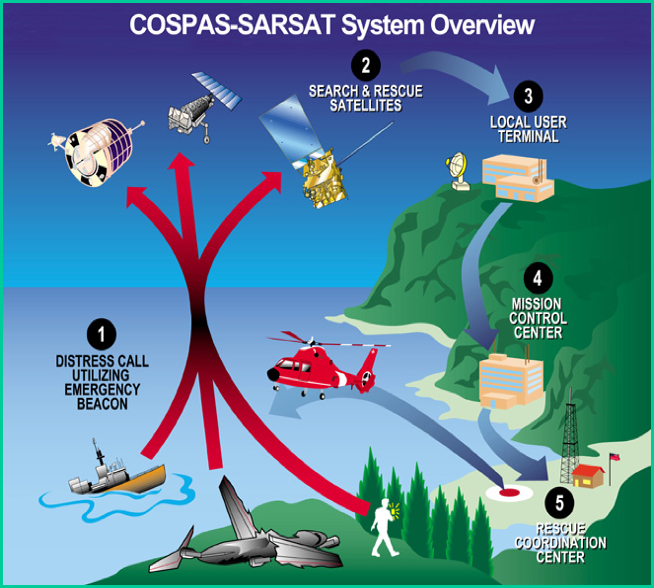
\includegraphics[width=6in]{diagram}
\caption[Search \& Rescue in action!]{Search \& Rescue in action!}%
\label{fig:sar-in-action}
\end{center}
\end{figure}

In standard GPS, a satellite in geosynchronous earth orbit emits a
constant frequency to let a receiver know his position.

In the old system (SARSAT) as well as the new (DASS) the satellites
relay distress-signal info (see below) to help a third party (the
rescuers) quickly determine a party in distress.


\section{\ldots{}and the New}%
\label{sec:new-system}

The proposed multi-satellite system (DASS) utilizes frequency of
arrival (FOA) and time of arrival (TOA) information from several
satellites for a location fix.� This results in near-instantaneous
beacon detection, since global coverage is continuous.� To improve the
system, a new algorithm for solving the required polynomial equations
is being implemented and tested.�


\section{Our Task/Deliverables}%
\label{sec:deliverables}

Our task was to implement in MATLAB an algorithm proposed by Cornell
computer scientist S.A. Vavasis that uses classical algebraic geometry
to solve the system of equations determined by two or more satellites,
and to analyze the algorithm�s stability and efficiency, and conduct a
literature search for possible alternative solution methods.

All deliverables were completed on schedule.

\section{Deriving the Equations}%
\label{sec:deriving-eqs}

We are interested in the situation when the beacon is observed by only
two satellites, since this case is ambiguous in the sense that there
are more than one possible location for the beacon position. To model
this situation, we will need five variables:
\begin{itemize}
\item $x$, $y$, and $z$, the coordinates of the beacon (sometimes
  these coordinates are referred to as the single vector $x$)

\item $t$, the time at which the distress signal is emitted

\item $f$, the frequency of the signal
\end{itemize}

The beacons used in the distress-alerting transmitters operate
nominally at a frequency of 406 megahertz, but small variations caused
by Doppler shifting (in many cases on the order of one-tenth of a
hertz). Atmospheric signal distortion requires us to treat $f$ as a
variable.

Our goal is to solve for the beacon location vector $x$, but the two
extra variables are needed so that the following system of five
equations is solvable.  Each satellite that receives a distress signal
is capable of measuring and recording its own location, the time of
the beacon signal�s detection, and the frequency of the incoming
signal, which we will denote as $s_{i}$, $t_{i}$, and $f_{i}$,
respectively (the subscript $i$ is used to distinguish the
satellites).

Our first two equations are the Time of Arrival equations, denoted
TOA1 and TOA2 (one each for $i = 1, 2$):
\begin{equation}
| x � s_{i} | = c ( t_{i} � t )
\end{equation}

The TOA equations simply relate the distance between the beacon and
the satellite to the time it takes for the signal to reach the
satellite ($c$ represents the speed of light).

The next pair of equations relates the observed frequency shift with
the relative velocity between the beacon and the satellite. These
equations are called the Frequency of Arrival equations FOA1 and FOA2:
\begin{equation}
 ( | x � s_{i}  |)' = w ( f_{i} � f )
\end{equation}

Here $w$ represents the nominal wavelength of the distress signal and
differentiation on the left side is with respect to time.

Finally, we assume that the beacon location is on the surface of the
earth and that the earth may be approximated by an ellipsoid. This
results in the following equation:
\begin{equation}
x Q xT  = 1
\end{equation}

This equation, denoted ALT, uses the diagonal matrix $Q$ to scale the
axes of the ellipsoid to match those of the earth.

These five equations---TOA1, TOA2, FOA1, FOA2, ALT---are all quadratic
in $x$, $t$, and $f$, and so, in principle, we have enough information
to solve for the beacon location.

\section{The Algorithm}%
\label{sec:the-algorithm}

Vavasis� algorithm allows us to use algebraic geometry to turn a
system of polynomial equations into an eigenvalue problem that we can
solve in MATLAB. The resultant matrix of a system of polynomials is a
sparse (mostly empty) matrix containing the coefficients of our
polynomials.

The steps of our algorithm are as follows:
\begin{itemize}
\item Given a system of equations $p_{1}, p_{2}, \dots, p_{k}$ in $n$
  variables, introduce an extra variable $x_{0}$ to make all the
  polynomials homogeneous.

\item Introduce an extra equation $q$ that is linear in the $n + 1$
  variables but whose coefficients are defined as $c_{i} = j_{i} + E
  k_{i}$, where the $j_{i}$ and $k_{i}$ are randomly chosen
  floating-point numbers and $E$ is the eigenvalue we hope to compute.

\item Create the large resultant matrix $M$ for the homogeneous
  system.

\item $M$ will not be square, so in order to create a sensible
  eigenvalue problem, we need to modify $M$:
  \begin{itemize}
  \item Delete specific rows of $M$ to create the square submatrix
    $N$, which we can write as the sum of two matrices $A$ and $E B: N
    = A + E B$.
  \item Use MATLAB to solve the generalized eigenvalue problem
    \begin{equation}
      (A + E B ) v = 0,
    \end{equation}
    and return $v$.
  \end{itemize}
\item In the eigenvector $v$ set $x_{0} = 1$ and take ratios of
  components to retrieve $x_{i}$-values that satisfy $p_{i}( x_{1},
  \dots , x_{n} ) = 0$.
\end{itemize}

This method of solving systems of polynomials has been known for a
hundred years, but has not been feasible until very recently, since
solving the generalized eigenvalue problem on large matrices is not
achievable by hand.

Due to the computational limitations of MATLAB (and computer algebra
systems in general) it is impossible for us to solve for $E$ and the
$x_{i}$ without introducing round-off error, so it is important that
we delete the rows of $M$ that will result in as stable a matrix $N$
as possible.

Vavasis� method uses QR-factorization to create a permutation matrix
that determines which rows of $M$ are to be deleted. All the rows
deleted relate to the adjoined polynomial $q$.  Vavasis proves certain
general bounds on the accuracy of his algorithm.  The method we have
chosen dates back to B.L.~van~der~Waerden (1903-�1996).  This method
deletes rows from potentially all but one of the polynomials $p_{1},
\dots , p_{n}, q$, and is known to be accurate.




\section{References}%
\label{sec:references}

Our literature search uncovered dozens of papers related to the study
of systems of polynomial equations. The two papers chiefly used in our
clinic project were:
\begin{itemize}
\item S.A.~Vavasis and G.F.~Jonsson. ``Accurate Solution of Polynomial
  Equations Using Macaulay Resultant Matrices''. 2001.
\item Jeff Mason. ``Algebraic Two-Satellite TOA/FOA Position Solution
  on an Ellipsoidal Earth''. Sandia National Laboratories. 2001.
\end{itemize}


\section{A Sample Run}%
\label{sec:sample-run}

The resultant matrix $M$ contains several rows for each of the $k + 1$
polynomials in our modified system and one column for each monomial of
degree $( d_{1} + \dots + d_{k} ) + (2 - k)$, where $d_{i}$ is the
degree of polynomial $p_{i}$.
 
For the system
\begin{equation}
x^{2} + y + z - 1 = 0\\
x + y^{2} + z - 1 = 0\\
x + y + z^{2} - 1 = 0
\end{equation}
we introduce the extra variable $w$ to obtain the homogeneous system
\begin{equation}
x^{2} + yw + zw - w^{2} = 0\\
xw + y^{2} + zw - w^{2} = 0\\
xw + yw + z^{2} - w^{2} = 0.
\end{equation}

The $\beta_{i}$ generated by MATLAB for the fourth equation,
\begin{equation}
c_{1}x + c_{2}y + c_{3}z + c_{4}w = 0
\end{equation}
were 0.1389, 0.2028, 0.1987, 0.6038, and so we see them in $B$, shown
in Figure~\ref{fig:big-matrix}.

\begin{figure}
\begin{center}
\resizebox*{9in}{!}{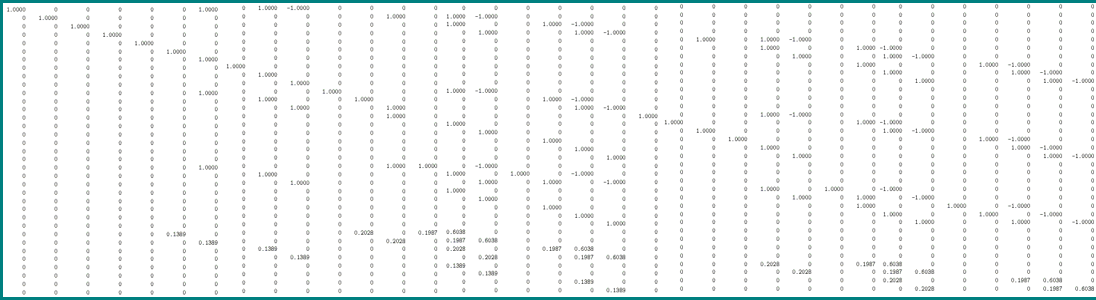
\includegraphics{big-matrix}}
\caption{The matrix $B$.}%
\label{fig:big-matrix}
\end{center}
\end{figure}

The matrix $B$ is 35 $\times$ 35 (down from $M$�s original 50 $\times$
35), and now we can finally solve for $E$ and $v$:
\begin{center}
  \begin{alltt}
    \fontsize{18pt}{22pt}\selectfont
    F = [poly2mat( [ 1 1 1 -1 ], [ 2 0 0; 0 1 0; 0 0 1; 0 0 0 ], 4, 2 );
    poly2mat( [ 1 1 1 -1 ], [ 1 0 0; 0 2 0; 0 0 1; 0 0 0 ], 4, 2 );
    poly2mat( [ 1 1 1 -1 ], [ 1 0 0; 0 1 0; 0 0 2; 0 0 0 ], 4, 2 ) ];
  \end{alltt}
\end{center}

Our program takes in the coefficients and degree sequences for the
three original polynomials, calculates $M$, $N$, $A$, and $B$ ($B$ is
shown in Figure~\ref{fig:big-matrix}), and returns the solution matrix
shown in Table~\ref{tab:solution-matrix}, corresponding to the
complete solution set shown in Table~\ref{tab:solution-set}.

\begin{table}
\begin{center}
\subfloat[Solution matrix.]%
{\begin{tabular}{lll}
-2.4142  &  -2.4142  & -2.4142\\
-0.0000  &  -0.0000  &  1.0000\\
 0.0000  &   0.0000  &  1.0000\\
 0.4142  &   0.4142  &  0.4142\\
 1.0000  &  -0.0000  & -0.0000\\
 1.0000  &   0.0000  &  0.0000\\
 0.0000  &   1.0000  &  0.0000\\
-0.0000  &   1.0000  & -0.0000
\end{tabular}%
\label{tab:solution-matrix}}
\qquad
\subfloat[Solution set.]%
{\begin{tabular}{@{(}l@{.}r@{, }l@{.}r@{, }l@{.}r@{)}}
-2 & 4142  &  -2 & 4142  & -2 & 4142\\
-0 & 0000  &  -0 & 0000  &  1 & 0000\\
 0 & 0000  &   0 & 0000  &  1 & 0000\\
 0 & 4142  &   0 & 4142  &  0 & 4142\\
 1 & 0000  &  -0 & 0000  & -0 & 0000\\
 1 & 0000  &   0 & 0000  &  0 & 0000\\
 0 & 0000  &   1 & 0000  &  0 & 0000\\
-0 & 0000  &   1 & 0000  & -0 & 0000
\end{tabular}%
\label{tab:solution-set}}
\caption{Solution.}%
\label{tab:solution}
\end{center}
\end{table}


\section{Acknowledgments}%
\label{sec:acknowledgments}

The Sandia math clinic team consisted of Todd CadwalladerOlsker,
Elizabeth Millan, Andy Niedermaier, Josh Padgett, and Luke Finlay
(fall 2003). Our team leader was Prof.~Weiqing Gu and our liaison at
Sandia National Laboratories was Dr.~Louis Romero.

We would like to thank Prof.~Gu and Dr.~Romero, as well as Jeff Mason
at Sandia, for their support, help, and direction throughout the
entire clinic project. We would also like to thank Prof.~Mike Raugh as
well as Barbara Schade for their assistance and advice in all
administrative aspects of the clinic project.

\end{poster}

\end{document}

 
